\chapter{Floating point arithmetic}%
\label{cha:rounding_errors}
\minitoc

\section*{Introduction}%
\label{sec:introduction}
% In numerical simulation,
% errors arise from four distinct sources:
% \begin{itemize}
%     \item
%         The \emph{modeling error} accounts for the mismatch between reality and the mathematical equations describing it.
%         Mathematical equations are generally only an approximation of reality.
%     \item
%         The \emph{numerical error}
%         refers to the error introduced by numerical methods,
%         which are generally not exact;
%         they only provide approximate solutions to the mathematical equations.
%     \item
%         The \emph{roundoff errors} come from the fact that
%         computers are unable to store the majority of real numbers exactly.
%         The number $\pi$, for example,
%         contains an infinite amount of digits
% \end{itemize}

When we study numerical algorithms in the next chapters,
we assume implicitly that the operations involved are performed exactly.
On a computer, however, only a subset of the real numbers can be stored and,
consequently, many arithmetic operations are performed only approximately.
This is the source of the so-called \emph{round-off errors}.
The rest of this chapter is organized as follows.
\begin{itemize}
    \item
        In \cref{sec:binary_representation_of_real_numbers},
        we discuss the binary representation of real numbers.

    \item
        In \cref{sec:set_of_values},
        we describe the set of floating point numbers that can be represented in the usual floating point formats;

    \item
        In \cref{sec:arithmetic_operations_between_floating_point_formats}
        we explain how arithmetic operations between floating point numbers behave.
        We insist in particular on the fact that,
        in a calculation involving several successive arithmetic operations,
        the result of each intermediate operation is stored as a floating point number,
        with a possible error.

    \item
        In \cref{sec:encoding_of_floating_point_numbers},
        we briefly present how floating point numbers are encoded
        according to the IEEE 754 standard, widely accepted today.
        We discuss also the encoding of special values such as \texttt{Inf}, \texttt{-Inf} and \texttt{NaN}.

    \item
        Finally, in \cref{sec:what_about_integer_formats},
        we present the standard integer formats and their encoding.
\end{itemize}
In order to completely describe floating-point arithmetic,
one would in principle need to also discuss the conversion mechanisms between different number formats,
as well as a number of edge cases.
% For instance, the reference IEEE 754 standard specifies that \texttt{NaN == NaN} must evaluate to \texttt{false},
% which is somewhat arbitrary but may be useful in some situations.
Needless to say,
a comprehensive discussion of the subject is beyond the scope of this course;
our aim in this chapter is only to introduce the key concepts.

\section{Binary representation of real numbers}%
\label{sec:binary_representation_of_real_numbers}

Given any integer number $\beta > 0$, called the \emph{base},
a real number $x$ can always be expressed as a finite or infinite series of the form
\begin{equation}
    \label{eq:base_representation}
    x = \pm \sum_{k=-n}^{\infty} a_k \beta^{-k}, \qquad a_k \in \{0, \dotsc, \beta - 1\}.
\end{equation}
The number $x$ may then be denoted as $\pm (a_{-n} a_{-n+1}\dots a_{-1} a_{0}.a_{1} a_{2} \dots)_{\beta}$,
where the subscript $\beta$ indicates the base.
This numeral system is called the \emph{positional notation} and is universally used today,
both by humans (usually with $\beta=10$) and machines (usually with $\beta=2$).
If the base~$\beta$ is omitted,
it is always assumed in this course that $\beta = 10$ unless otherwise specified
-- this is the \emph{decimal} representation.
The \emph{digits} $a_{-n}, a_{-n+1}, \dotsc$ are also called \emph{bits} if $\beta = 2$.
In computer science, several bases other than 10 are regularly employed,
for example the following:
\begin{itemize}
    \item
        Base 2 (binary) is the usual choice for storing numbers on a machine.
        The binary format is convenient because the digits have only two possible values, 0 or 1,
        and so they can be stored using simple electrical circuits with two states.
        We employ the binary notation extensively in the rest of this chapter.
        Notice that, just like multiplying and dividing by~10 is easy in base 10,
        multiplying and dividing by 2 is very simple in base 2:
        these operations amount to shifting all the bits by one position to the left or right,
        respectively.

    \item
        Base 16 (hexadecimal) is sometimes convenient to represent numbers in a compact manner.
        In order to represent the values 0-15 with a single digit,
        16 different symbols are required, which are conventionally denoted by $\{0,1,2,3,4,5,6,7,8,9,A,B,C,D,E,F\}$.
        With this notation, we have $(FF)_{16} = (255)_{10}$, for example.

        The hexadecimal notation is often used in programming languages for describing colors specified by a triplet $(r,g,b)$ of values between 0 and 255,
        corresponding to the primary colors \emph{red}, \emph{blue} and \emph{green}.
        The number of possible values for each component is~$256 = 16^2$,
        and so only 2 digits are required to represent these in the hexadecimal notation.
        Hexadecimal numbers are also employed in IPv6 addresses,
        which are used to identify computers connected to a network.
\end{itemize}

\subsection{Conversion between binary and decimal formats}%
Obtaining the decimal representation of a binary number can be achieved from~\eqref{eq:base_representation},
using the decimal representations of the powers of 2.
Since all the positive and negative powers of 2 have a finite decimal representation,
any real number with a finite representation in base 2 has a finite representation also in base 10.
For example, $(0.01)_2 = (0.25)_{10}$ and $(0.111)_2 = (0.875)_{10}$.
\begin{example}
    [Converting a binary number to decimal notation]
    \label{example:converting_binary_to_decimal}
    Let us calculate the decimal representation of $x = (0.\overline{10})_2$,
    where the horizontal line indicates repetition: $x = (0.101010\dots)_2$.
    By definition, it holds that
    \[
        x = \sum_{k=0}^{\infty} a_k 2^{-k},
    \]
    where $a_k = 0$ if $k$ is even and 1 otherwise.
    Thus, the series may be rewritten as
    \[
        x = \sum_{k=0}^{\infty} 2^{-(2k+1)} = \frac{1}{2} \sum_{k=0}^{\infty} (2^{-2})^k.
    \]
    We recognize on the right-hand side a geometric series with common ratio $r = 2^{-2} = \frac{1}{4}$,
    and so we obtain
    \[
        x = \frac{1}{2} \left( \frac{1}{1-r} \right) = \frac{2}{3} = (0.\overline 6)_{10}.
    \]
\end{example}

Obtaining the binary representation of a decimal number is more difficult,
because negative powers of 10 have \emph{infinite} binary representations,
as \cref{exercise:binary_zero_point_one} demonstrates.
There is, however, a simple procedure to perform the conversion,
which we present for the specific case of a real number $x$ with decimal representation of the form $x = (0.a_1\dots a_n)_{10}$.
In this setting,
the bits~$(b_1, b_2, \dots)$ in the binary representation of $x = (0.b_1b_2b_2 \dots)_2$ may be obtained as follows:
\begin{algorithm}
\caption{Conversion of a number to binary format}%
\label{algo:conversion_to_binary}%
\begin{algorithmic}[1]
\State $i \gets 1$
\While{$x \neq 0$}
    \State $x \gets 2x$%
    \label{line:after_while}
    \If{$x \geq 1$}
        \State $b_i \gets 1$
    \Else
        \State $b_i \gets 0$
    \EndIf
    \State $x \gets x - b_i$
    \State $i \gets i+1$
\EndWhile
\end{algorithmic}
\end{algorithm}

\begin{example}
    [Converting a decimal number to binary notation]
    Let us calculate the binary representation of $x = \frac{1}{3} = (0.\overline{3})_{10}$.
    We apply~\cref{algo:conversion_to_binary} and collate the values of $i$ and $x$ obtained at the beginning of each iteration,
    i.e.\ just before~\cref{line:after_while}, in the table below.
    \begin{center}
    \begin{tabular}{|c|c|c|}
        \hline
        $i$ & $x$ & Result \\ \hline
        $1$ & $\frac{1}{3}$ & 0.\textbf{0}000\dots \\ \hline
        $2$ & $\frac{2}{3}$ & 0.0\textbf{1}00\dots \\ \hline
        $3$ & $\frac{1}{3}$ & 0.00\textbf{0}0\dots \\ \hline
    \end{tabular}
    \end{center}
    Since $x$ in the last row is again $\frac{1}{3}$,
    successive bits alternate between 0 and 1,
    and the binary representation of $x$ is given by $(0.\overline{01})_2$.
    This is not surprising since $2x = (0.66)_{10} = (0.\overline{10})_2$,
    as we saw in~\cref{example:converting_binary_to_decimal}.
\end{example}

\subsection{Exercises}%

\begin{exercise}
    \label{exercise:non_unique_representation}
    Show that if a number $x \in \real$ admits a finite representation~\eqref{eq:base_representation} in base~$\beta$,
    then it also admits an infinite representation in the same base.
    \textbf{Hint:} You may have learned before that $(0.\overline 9)_{10} = 1$.
\end{exercise}

\begin{exercise}
    How many digits does it take to represent all the integers from 0 to $10^{10} - 1$ in decimal and binary format?
    What about the hexadecimal format?
\end{exercise}

\begin{exercise}
    Find the decimal representation of $(0.000\overline{1100})_2$.
\end{exercise}

\begin{exercise}
    \label{exercise:binary_zero_point_one}
    Find the binary representation of $(0.1)_{10}$.
\end{exercise}

\begin{compexercise}
    Implement~\cref{algo:conversion_to_binary} on a computer and verify that it works.
    Your function should take as argument an array of integers containing the digits after the decimal point;
    that is, an array of the form \verb?[a_1, ..., a_n]?.
\end{compexercise}

\begin{compexercise}
    As mentioned above, \cref{algo:conversion_to_binary} works only for decimal numbers of the specific form~$x = (0.a_1\dots a_n)_{10}$.
    Find and implement a similar algorithm for integer numbers.
    More precisely, write a function that takes an integer $n$ as argument and
    returns an array containing the bits of the binary expansion $(b_m \dots b_0)_2$ of $n$,
    from the least significant $b_0$ to the most significant $b_m$.
    That is to say, your code should return \mintinline{julia}{[b_0, b_1, ...]}.
    \begin{minted}{julia}
    function to_binary(n)
        # Your code comes here
    end

    # Check that it works
    number = 123456789
    bits = to_binary(number)
    pows2 = 2 .^ range(0, length(bits) - 1)
    @assert sum(bits'pows2) == number
    \end{minted}
\end{compexercise}

\section{Set of values representable in floating point formats}%
\label{sec:set_of_values}
We mentioned in the introduction that,
because of memory limitations,
only a subset of the real numbers can be stored exactly in a computer.
Nowadays, the vast majority of programming languages and software comply with the IEEE 754 standard,
which requires that the set of representable numbers be of the form
\begin{align}
    \notag
    \floating (p, E_{\min}, E_{\max})
    = \Bigl\{ & (-1)^s 2^E (b_0. b_1 b_2 \dots b_{p-1})_2 \colon \\
    \label{eq:number_format}%
              & \qquad s \in \{0, 1\}, b_i \in \{0, 1\} \, \text{and} \, E_{\min} \leq E \leq E_{\max} \Bigr\}.
\end{align}
In addition to these, floating number formats provide the special entities \texttt{Inf}, \texttt{-Inf} and \texttt{NaN},
the latter being an abbreviation for \emph{Not a Number}.
Three parameters appear in the set definition~\eqref{eq:number_format}.
The parameter $p \in \nat_{>0}$ is the number of significant bits (also called the precision),
and $(E_{\min}, E_{\max}) \in \integer^2$ are respectively the minimum and maximum exponents.
From the precision, the \emph{machine epsilon} is defined as $\varepsilon_{M} = 2^{-p-1}$;
its significance is discussed in~\cref{sub:relative_error_and_epsilon_machine}.

For a number $x \in \floating(p, E_{\min}, E_{\max})$,
$s$ is called the \emph{sign}, $E$ is the \emph{exponent} and
$b_0. b_1 b_2 \dots b_{p-1}$ is the \emph{significand}.
The latter can be divided into a \emph{leading bit} $b_0$ and the \emph{fraction} $b_1 b_2 \dots b_{p-1}$,
to the right of the binary point.
The most widely used floating point formats are the \emph{single} and \emph{double precision} formats,
which are called respectively \julia{Float32} and \julia{Float64} in Julia.
Their parameters,
together with those of the lesser-known half-precision format,
are summarized in~\cref{table:floating_point_formats}.
In the rest of this section we use the shorthand notation $\floating_{16}$, $\floating_{32}$ and $\floating_{64}$.
Note that $\floating_{16} \subset \floating_{32} \subset \floating_{64}$.
\begin{table}[ht]
    \centering
    \begin{tabular}{|c|c|c|c|}
        \hline
        & Half precision & Single precision & Double precision
        \\ \hline
        $p$ & 11 & 24 & 53
        \\ \hline
        $E_{\min}$ & -14 & -126 & -1022
        \\ \hline
        $E_{\max}$ & 15 & 127 & 1023
        \\ \hline
    \end{tabular}
    \caption{%
        Floating point formats.
        The first column corresponds to the \emph{half-precision} format.
        This format,
        which is available through the \texttt{Float16} type in Julia,
        is more recent than the single and double precision formats.
        It was introduced in the 2008 revision to the IEEE 754 standard of 1985,
        a revision known as IEEE 754-2008.
    }%
    \label{table:floating_point_formats}
\end{table}

\begin{remark}
    Some definitions,
    notably that in~\cite[Section 2.5.2]{MR2265914},
    include a general base~$\beta$ instead of the base 2
    as an additional parameter in the definition of the number format~\eqref{eq:number_format}.
    Since the binary format ($\beta = 2$) is always employed in practice,
    we focus on this case for simplicity in most of this chapter.
\end{remark}

\begin{remark}
    \label{remark:roundoff_non_uniqueness}
    Given a real number $x \in \floating (p, E_{\min}, E_{\max})$,
    the exponent $E$ and significand  are generally not uniquely defined.
    For example, the number $2.0 \in \floating_{64}$ may be expressed as $(-1)^0 2^1 (1.00\dots00)_2$ or, equivalently, as $(-1)^0 2^{2} (0.100\dots00)_2$.
\end{remark}

In \texttt{Julia}, non-integer number literals are interpreted as \julia{Float64} by default,
which can be verified by using the \julia{typeof} function.
For example, the instruction ``\julia{a = 0.1}'' is equivalent to~``\julia{a = Float64(0.1)}''.
In order to define a number of type \julia{Float32},
the suffix $\julia{f0}$ must be appended to the decimal expansion.
For instance, the instruction ``$\julia{a = 4.0f0}$'' defines a floating point number~\julia{a} of type \julia{Float32};
it is equivalent to writing ``\julia{a = Float32(4.0)}''.

\subsection{Denormalized floating point numbers}%
\label{sub:defining_a_unique_representation}
We can decompose the set $\floating(p, E_{\min}, E_{\max})$ in two disjoint parts:
\begin{align*}
    \label{eq:decomposition_normalized_denormalized}%
    \floating (p, E_{\min}, E_{\max})
    &= \Bigl\{ (-1)^s 2^E (\textcolor{red}{1}. b_1 b_2 \dots b_{p-1})_2 \colon \\
    & \qquad s \in \{0, 1\}, b_i \in \{0, 1\} \, \text{and} \, E_{\min} \leq E \leq E_{\max} \Bigr\} \\
    &\qquad \cup \Bigl\{  (-1)^s 2^{\textcolor{red}{E_{\min}}} (\textcolor{red}{0}. b_1 b_2 \dots b_{p-1})_2 \colon
     s \in \{0, 1\}, b_i \in \{0, 1\} \Bigr\}.
\end{align*}
The numbers in the second set are called \emph{subnormal} or \emph{denormalized}.

\subsection{Relative error and machine epsilon}%
\label{sub:relative_error_and_epsilon_machine}
Let $x$ be a nonzero real number and $\widehat x$ be an approximation.
We define the absolute and relative errors of the approximation as follows.
\begin{definition}
    [Absolute and relative error]
    The absolute error is given by $|x - \widehat x|$,
    whereas the relative error is
    \[
        \frac{|x - \widehat x|}{|x|}
    \]
\end{definition}

The following result establishes a link between the machine $\varepsilon_M$ and
the relative error between a real number and the closest member of a floating point format.
\begin{proposition}
    \label{prop:relative_error_and_machine_epsilon}
    Let $x_{\min}$ and $x_{\max}$ denote the smallest and largest \emph{non-denormalized} positive numbers in a format $F = \floating(p, E_{\min}, E_{\max})$.
    If $x \in [-x_{\max}, -x_{\min}] \cup [x_{\min}, x_{\max}]$,
    then
    \begin{equation}
        \label{eq:bound_epsilon_machine}
        \min_{\widehat x \in F} \frac{|x - \widehat x|}{|x|} \leq \frac{1}{2} 2^{-(p-1)}
        = \frac{1}{2} \varepsilon_M.
    \end{equation}
\end{proposition}
\begin{proof}
    For simplicity, we assume that $x > 0$.
    Let $n = \lfloor \log_2(x) \rfloor$ and $y := 2^{-n} x$.
    Since $y \in [1, 2)$,
    it admits a binary representation of the form
    \(
        (1.b_1 b_2\dots)_2 \neq (1.\overline 1)_2
    \)
    Thus
    \(
        x = 2^{n} (1.b_1 b_2\dots)_2,
    \)
    and from the assumption that $x_{\min} \leq x \leq x_{\max}$
    we deduce that $E_{\min} \leq n \leq E_{\max}$.
    % \footnote{%
    %     The inequality here is strict,
    %     because $2^{E_{\min} - 1} (1.\overline{1})_2 = 2^{E_{\min}} = x_{\min}$.
    %     Remember that the binary expansion of a real number is generally not unique!
    %     See~\cref{exercise:non_unique_representation}.
    % }
    % which is excluded by assumption.
    We now define the number $x_- \in F$ by truncating the binary expansion of $x$ as follows:
    \[
        x_- = 2^n (1.b_1 \dots b_{p-1})_2.
    \]
    The distance between $x_-$ and its successor in $F$,
    which we denote by $x_+$, is given by $2^{n-p+1}$.
    Consequently, it holds that
    \[
        (x_+ - x) + (x-x_-) = x_+ - x_- = 2^{n-p+1}.
    \]
    Since both summands on the left-hand side are positive,
    this implies that either $x_+ - x$ or $x - x_-$ is bounded from above by $\frac{1}{2} 2^{n-p+1} \leq \frac{1}{2} 2^{-p+1}x$,
    which concludes the proof.
\end{proof}

The machine epsilon,
which was defined as $\varepsilon_M = 2^{-(p-1)}$,
coincides with the maximum relative spacing between a non-denormalized floating point number $x$ and its successor in the floating point format,
defined as the smallest number in the format that is strictly larger than~$x$.

\Cref{fig:float64_density} depicts the density of double-precision floating point numbers,
i.e.\ the number of~$\floating_{64}$ members per unit on the real line.
The figure shows that the density decreases as the absolute value of $x$ increases.
We also notice that the density is piecewise constant with discontinuities at powers of 2.
\Cref{fig:float64_spacing} illustrates the relative spacing between successive floating point numbers.
Although the absolute spacing increases with the absolute value of $x$,
the relative spacing oscillates between~$\frac{1}{2} \varepsilon_{M}$ and~$\varepsilon_M$.

\begin{figure}
    \centering
    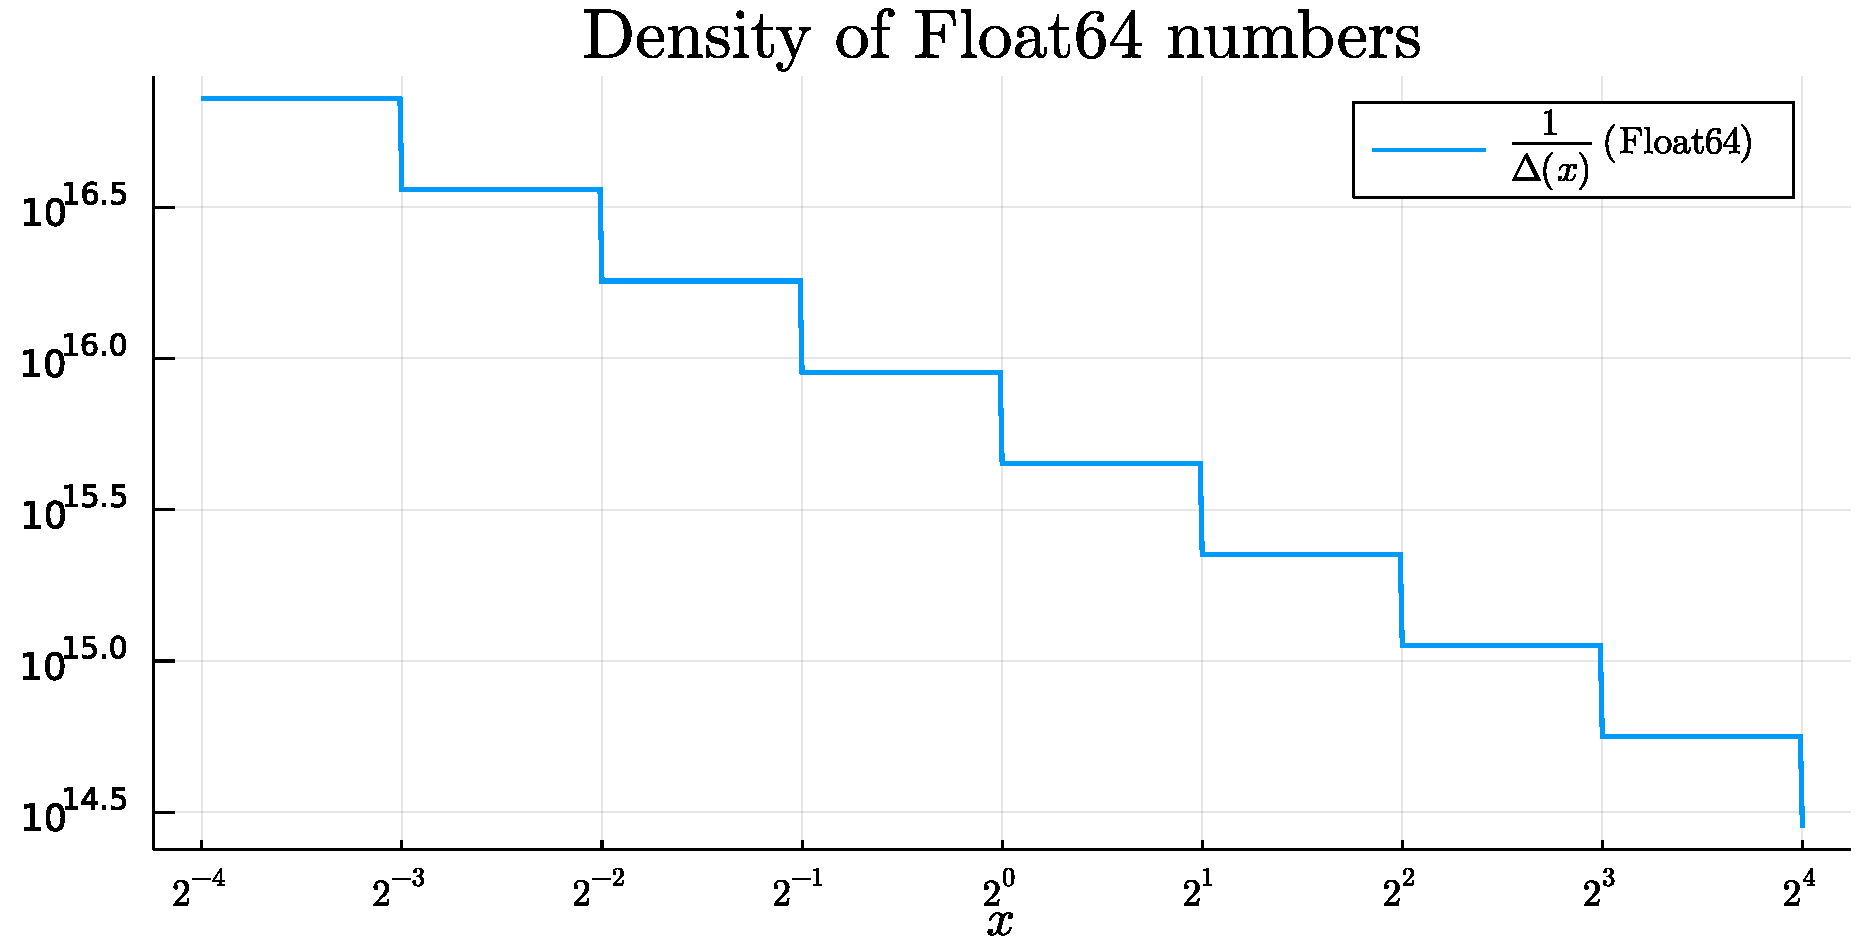
\includegraphics[width=.8\textwidth]{figures/float64_density.pdf}
    \caption{%
        Density of the double-precision floating point numbers,
        measured here as~$1/\Delta(x)$ where,
        for $x \in \floating_{64}$,
        $\Delta(x)$ denotes the distance between $x$ and its successor in $\floating_{64}$.
    }%
    \label{fig:float64_density}%
\end{figure}

\begin{figure}[ht]
    \centering
    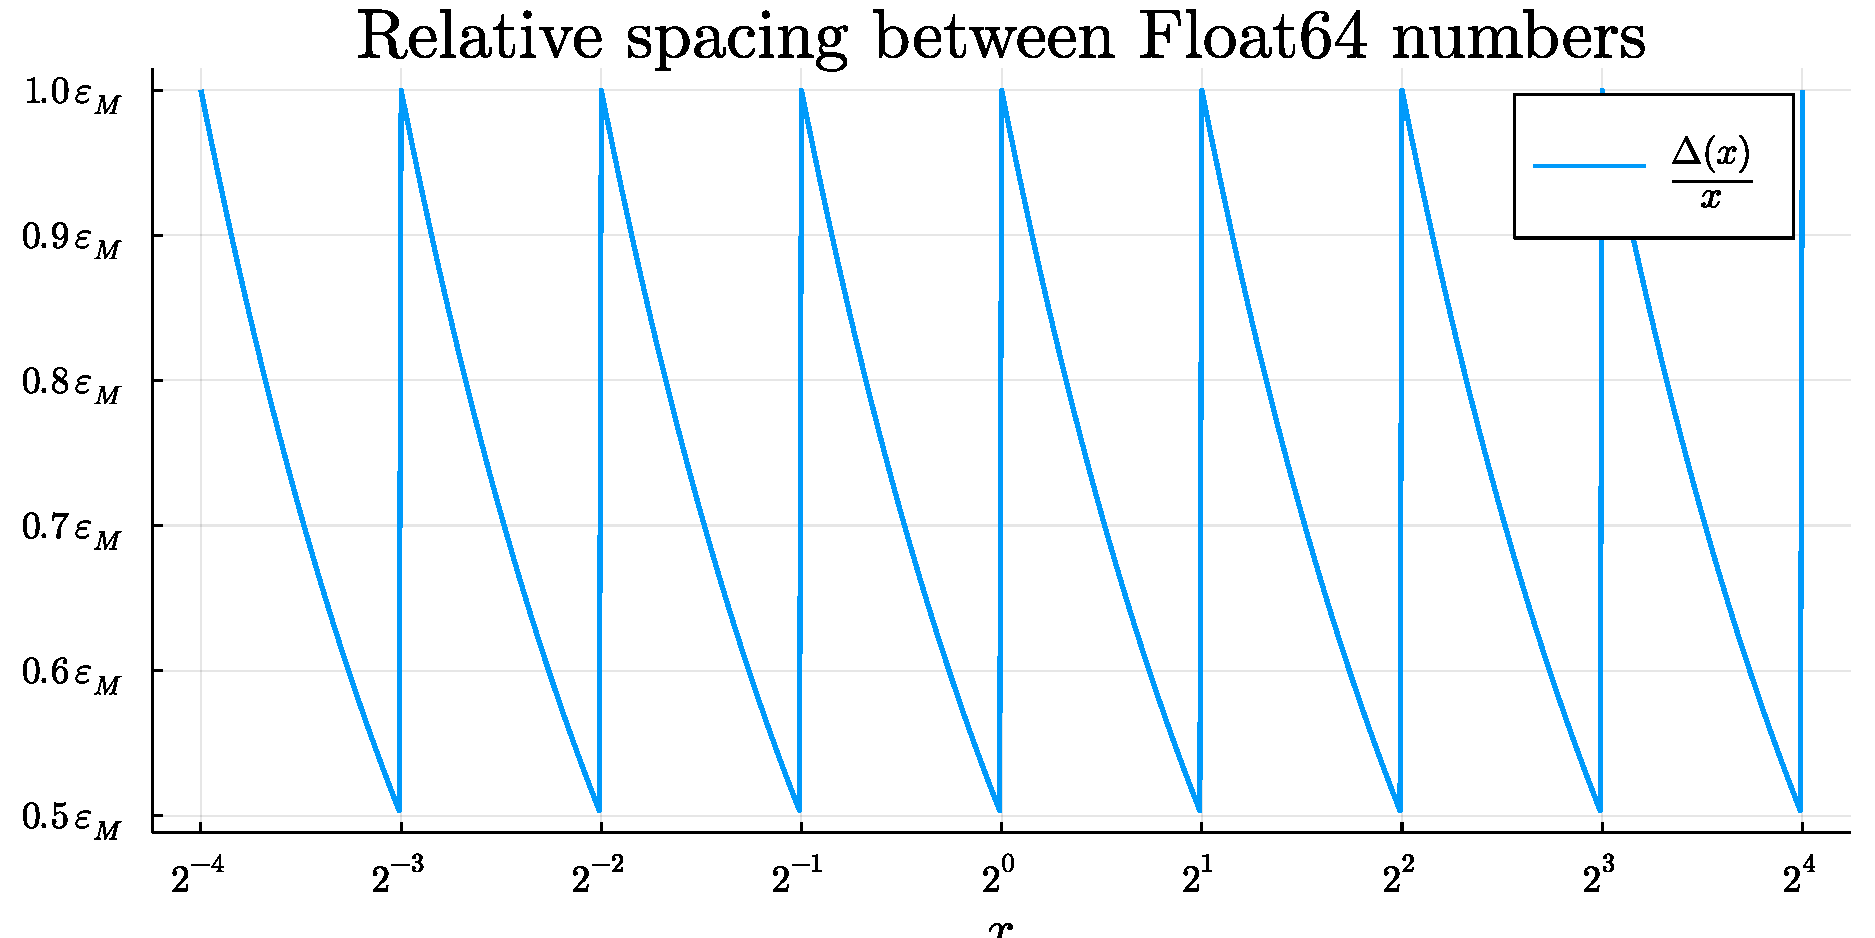
\includegraphics[width=.65\textwidth]{figures/float64_spacing.pdf}
    \caption{%
        Relative spacing between successive double-precision floating point numbers in the ``normal range''.
        The relative spacing oscillates between $\frac{1}{2} \varepsilon_M$ and $\varepsilon_M$.
    }%
    \label{fig:float64_spacing}
\end{figure}

The picture of the relative spacing between successive floating point numbers looks quite different for denormalized numbers.
This is illustrated in \cref{fig:float64_spacing_denormalized},
which shows that the relative spacing increases beyond the machine epsilon in the denormalized range.
Fortunately, in the usual $\floating_{32}$ and $\floating_{64}$ formats,
the transition between denormalized and non-denormalized numbers occurs at such a small value that
it rarely needs worrying about.

\begin{figure}[ht]
    \centering
    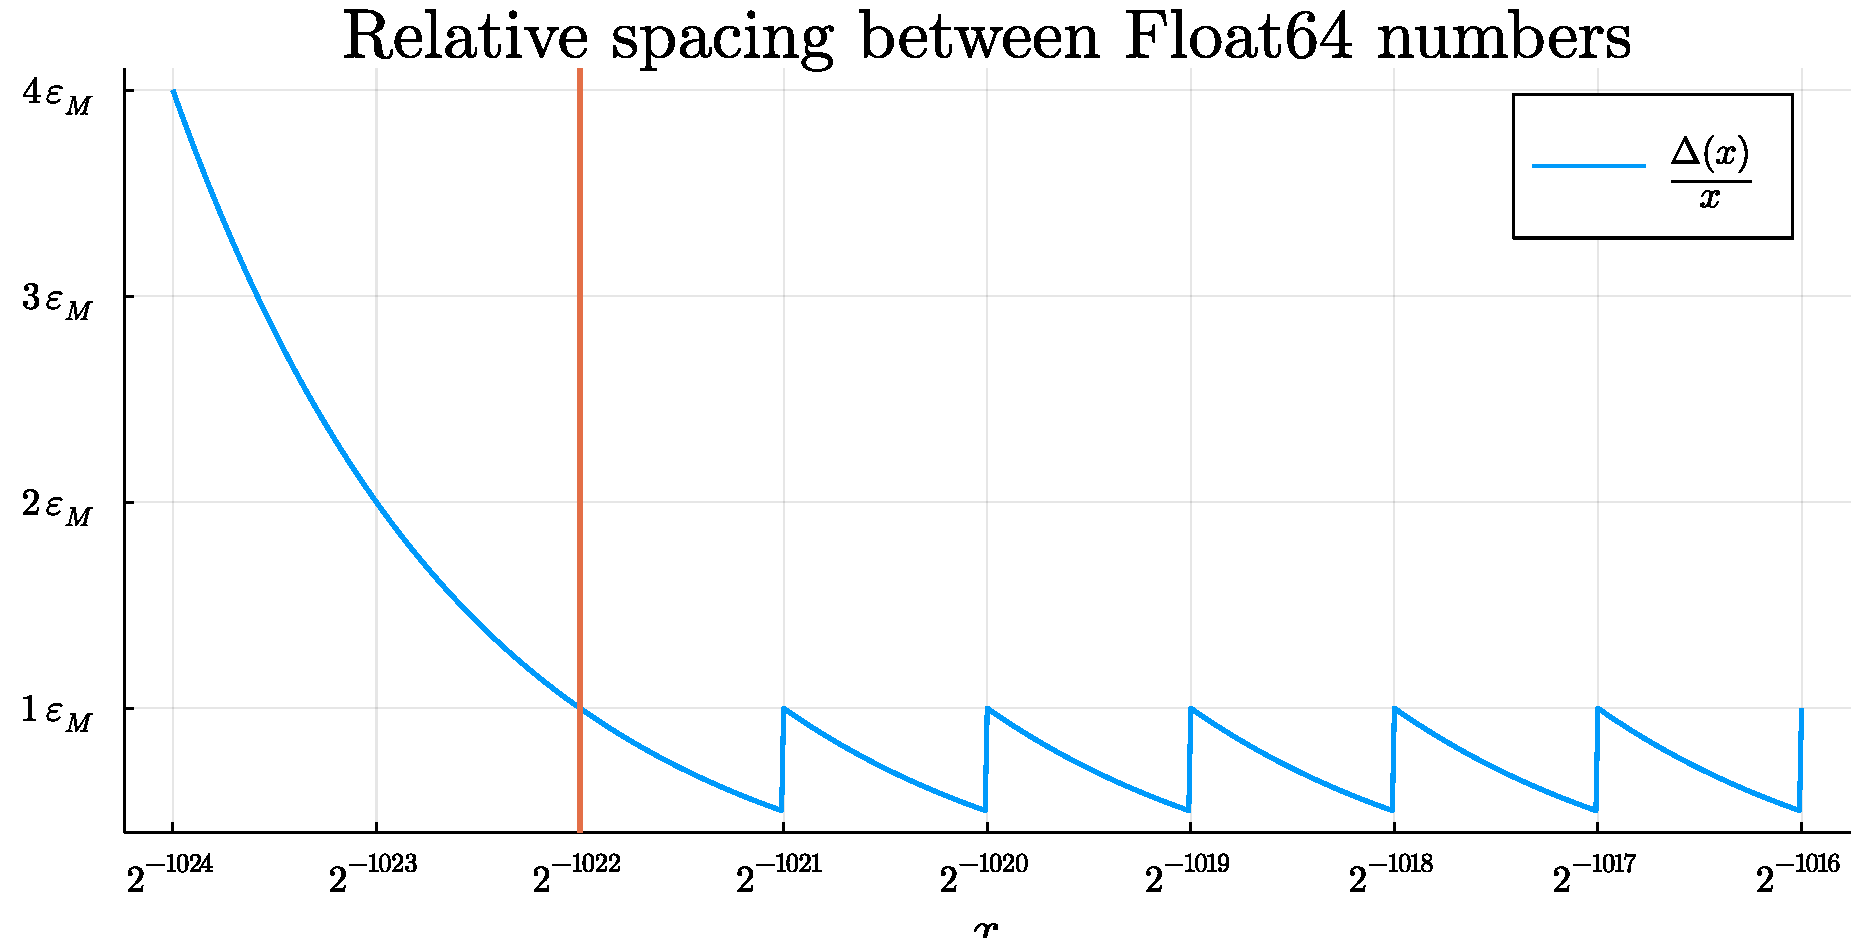
\includegraphics[width=.65\textwidth]{figures/float64_spacing_denormalized.pdf}
    \caption{%
        Relative spacing between successive double-precision floating point numbers,
        over a range which includes denormalized number.
        The vertical red line indicates the transition from denormalized to non-denormalized numbers.
    }%
    \label{fig:float64_spacing_denormalized}
\end{figure}

\begin{example}
    In Julia,
    the machine epsilon can be obtained using the \texttt{eps} function.
    For example, the instruction \julia{eps(Float16)} returns $\varepsilon_M$ for the half-precision format.
\end{example}

\subsection{Exercises}%

\begin{exercise}
    Show that the successor of $1$ in $\floating_{64}$ is $1 + \varepsilon_M$,
    where $\varepsilon_M$ is the machine epsilon for the double-precision format.
\end{exercise}

\begin{exercise}
    Write down the values of the smallest and largest, in absolute value,
    positive real numbers representable in the $\floating_{32}$ and $\floating_{64}$ formats.
\end{exercise}

\begin{exercise}
    [Relative error and machine epsilon]
    \label{exercise:machine_epsilon}
    Prove that the inequality~\eqref{eq:bound_epsilon_machine} is sharp.
    To this end, find $x \in \real$ such that the inequality is an equality.
\end{exercise}

\begin{exercise}
    [Cardinality of the set of floating point numbers]
    \label{exercise:cardinality_floating}
    Show that, if $E_{\max} \geq E_{\min}$, then $\floating(p, E_{\min}, E_{\max})$ contains exactly
    \[
        (E_{\max} - E_{\min}) 2^{p} + 2^{p+1} - 1
    \]
    \emph{distinct real numbers}.
    (In particular, the special values \texttt{Inf}, \texttt{-Inf} and \texttt{NaN} are not counted.)
    \textbf{Hint:} Count first the numbers with $E > E_{\min}$ and then those with $E = E_{\min}$.
\end{exercise}

\section{Arithmetic operations between floating point formats}%
\label{sec:arithmetic_operations_between_floating_point_formats}

Now that we have presented the set of values representable on a computer,
we attempt in this section to understand precisely how arithmetic operations between floating point formats are performed.
The key mechanism governing arithmetic operations on a computer is that of \emph{rounding},
the action of approximating a real number regarded as infinitely precise by a number in a floating point format $\floating (p, E_{\min}, E_{\max})$.
The IEEE 754 standard stipulates that the default mechanism for rounding a real number $x$,
called \emph{round to nearest},
should behave as follows:
\begin{itemize}
    \item
        \textbf{Standard case}:
        The number $x$ is rounded to the \emph{nearest representable number},
        if this number is unique.
    \item
        \textbf{Edge case}:
        When there are two equally near representable numbers in the floating point format,
        the one with the least significant bit equal to zero is delivered.
    \item
        \textbf{Infinities}:
        If the real number $x$ is larger than the largest representable number in the format,
        that is larger than or equal to $x_{\max} = 2^{E_{\max}} (2 - 2^{-p-1})$,
        then there are two cases,
        \begin{itemize}
            \item If $x < 2^{E_{\max}} (2 - 2^{-p})$, then $x_{\max}$ is delivered;
            \item Otherwise, the special value~\texttt{Inf} is delivered.
        \end{itemize}
        In other words, $x_{\max}$ is delivered if it would be delivered by following the rules of the first two bullet points
        in a different floating point format with the same precision but a larger exponent $E_{\max}$.
        A similar rule applies for large negative numbers.
\end{itemize}

When a binary arithmetic operation ($+$, $-$, $\times$, $/$) is performed on floating point numbers in format $\floating$,
the result delivered by the computer is obtained by rounding the exact result of the operation according to the rules given above.
In other words,
the arithmetic operation is performed as if the computer first calculated an intermediate exact result,
and then rounded this intermediate result in order to provide a final result in $\floating$.

Mathematically,
arithmetic operations between floating point numbers in a given format $\floating$ may be formalized by introducing
the rounding operator ${\rm fl}: \real \to \floating$ and
by defining, for any binary operation $\circ \in \{+, -, \times, /\}$,
the corresponding machine operation
\[
    \widehat \circ\colon \floating \times \floating \rightarrow \floating; (x, y) \mapsto {\rm fl}(x \circ y).
\]
We defined this operator for arguments in the same floating point format~$\floating$.
If the arguments of a binary arithmetic operation are of different types,
the format of the end result,
known as the \emph{destination format},
depends on that of the arguments:
as a rule of thumb,
it is given by the most precise among the formats of the arguments.
In addition, recall that a floating point literal whose format is not explicitly specified is rounded to double-precision format
and so, for example, the addition \julia{0.1 + 0.1} produces the result ${\rm fl_{64}}\bigl(\rm fl_{64}(0.1) + \rm fl_{64}(0.1)\bigr)$,
where ${\rm fl}_{64}$ is the rounding operator to the double-precision format.

\begin{example}
    Using the \julia{typeof} function,
    we check that the floating point literal \texttt{1.0} is indeed interpreted as a double-precision number:
    % julia-repl does not work on old versions of LaTeX
% \begin{minted}{julia-repl}
\begin{minted}{julia}
julia> a = 1.0; typeof(a)
Float64
\end{minted}
When two numbers in different floating point formats are passed to a binary operation,
the result is in the more precise format.
% \begin{minted}{julia-repl}
\begin{minted}{julia}
julia> typeof(Float16(1) + Float32(1))
Float32

julia> typeof(Float32(1) + Float64(1))
Float64
\end{minted}
\end{example}

If a mathematical expression contains several binary arithmetic operations to be performed in succession,
the result of each intermediate calculation is stored in a floating point format dictated by the formats of its argument,
and this floating point number is employed in the next binary operation.
A consequence of this mechanism is that the machine operands $\madd$ and $\mtimes$ are generally \emph{not associative}.
For example, in general
\[
    (x \madd y) \madd  z \neq x \madd (y \madd z)
\]
\begin{example}
    Let $x = 1$ and $y = 3 \times 2^{-13}$.
    Both of these numbers belong to $\floating_{16}$ and,
    denoting by $\widehat +$ machine addition in~$\floating_{16}$,
    we have
    \begin{equation}
        \label{eq:non_associativity_1}
        (x \madd y) \madd y = 1
    \end{equation}
    but
    \begin{equation}
        \label{eq:non_associativity_2}
        x \madd (y \madd y) = 1 + 2^{-10}.
    \end{equation}
    To explain this somewhat surprising result,
    we begin by writing the normalized representations of~$x$ and $y$ in the $\floating_{16}$ format:
    \begin{align*}
        x &= (-1)^0 \times 2^0 \times (\texttt{1.0000000000})_2 \\
        y &= (-1)^0 \times 2^{-12} \times (\texttt{1.1000000000})_2.
    \end{align*}
    The exact result of the addition $x + y$ is given by $r = 1 + 3 \times 2^{-13}$,
    which in binary notation is
    \[
        r = (1.\underbrace{00000000000}_{\text{11 zeros}}11)_2.
    \]
    Since the length of the significand in the half-precision ($\floating_{16}$) format is only $p = 11$,
    this number is not part of $\floating_{16}$.
    The result of the machine addition $\madd$ is therefore obtained by rounding $r$ to the nearest member of~$\floating_{16}$,
    which is 1.
    This reasoning can then be repeated in order to conclude that, indeed,
    \[
        (x \madd y) \madd y = x \madd y = 1.
    \]

    In order to explain the result of~\eqref{eq:non_associativity_2},
    note that the exact result of the addition $y + y$ is $r = 3 \times 2^{-12}$,
    which belongs to the floating point format,
    so it also holds that $y \madd y = 3 \times 2^{-12}$.
    Therefore,
    \[
        x \madd (y \madd y) = 1 \madd 3 \times 2^{-12} = {\rm fl}_{16} (1 + 3 \times 2^{-12}).
    \]
    The argument of the $\floating_{16}$ rounding operator does not belong to $\floating_{16}$,
    since its binary representation is given by
    \[
        (1.\underbrace{0000000000}_{\text{10 zeros}}11)_2.
    \]
    This time the nearest member of $\floating_{16}$ is given by $1 + 2^{-10}$.
\end{example}

When a numerical computation unexpectedly returns \texttt{Inf} or \texttt{Inf},
we say that an \emph{overflow error} occurred.
Similarly, \emph{underflow} occurs when a number
is smaller than the smallest representable number in a floating point format.

\subsection{Exercises}%

% \begin{exercise}
%     [Tie to even]
%     Explain why,
%     in the $\floating_{16}$ format,
%     \[
%         1 \madd 2^{-10} \madd 2^{-11} = 1 \madd 2^{-10}
%     \]
%     but
%     \[
%         1 \madd 2^{-11} = 1 \madd 2^{-10}.
%     \]
% \end{exercise}

\begin{exercise}
    Calculate the machine epsilon $\varepsilon_{16}$ for the $\floating_{16}$ format.
    Write the results of the arithmetic operations $1 \madd \varepsilon_{16}$ and $1 \msub \varepsilon_{16}$ in the form
    \[
        2^E (1.b_1 \dotsc b_{p-1})_2.
    \]
\end{exercise}

\begin{exercise}
    Let $\varepsilon_{16}$ be the machine epsilon for the $\floating_{16}$ format,
    and define $y = \frac{4}{3} \varepsilon_{16}$.
    What is the relative error between $\Delta = (1 + y) - 1$,
    and the machine approximation $\widehat \Delta = (1 \madd y) \msub 1$?
\end{exercise}

\begin{compexercise}
    [Numerical differentiation]
    Let $f(x) = \exp(x)$.
    By definition, the derivative of~$f$ at~$0$ is
    \[
        f'(0) = \lim_{\delta \to 0} \left( \frac{f(\delta) - f(0)}{\delta} \right).
    \]
    The expression within brackets on the right-hand side may be used
    with a small but nonzero~$\delta$ as an approximation for $f'(0)$.
    Implement this approach using double-precision numbers and the same values for $\delta$ as in the table below.
    Explain the results you obtain.
    \begin{center}
        \def\arraystretch{1.5}
        \begin{tabular}{|c|c|c|c|}
            \hline
            $\delta$ & $\frac{\varepsilon_{64}}{4} $ & $\frac{\varepsilon_{64}}{2}$ & $\varepsilon_{64}$ \\
            \hline
            Approximation of $f'(0)$ & 0 & 2 & 1 \\
            \hline
        \end{tabular}
    \end{center}
\end{compexercise}

\begin{compexercise}
    [Numerical differentiation]
    Let $f(x) = \exp(x)$ and let \julia{d(δ)} be the approximation of $f'(0)$ given by
    \begin{minted}{julia}
        f(x) = exp(x)
        d(δ) = (f(0+δ) - f(0))/δ
    \end{minted}
    Plot \julia{d(δ)} as a function of~\julia{δ} in logarithmic scale and explain the result.
\end{compexercise}

\begin{compexercise}
    [Avoiding overflow]
    Write a code to calculate the weighted average
    \[
        S := \frac
        {\sum_{j=0}^{J} w_j j}
        {\sum_{j=0}^{J} w_j},
        \qquad w_j = \exp(j),
        \qquad J = 1000.
    \]
    You may need to first rewrite~$S$ differently.
\end{compexercise}

\begin{compexercise}
    Plot the function $x \mapsto \log\left(\e^{\e^x} - 1\right)$ over the interval $[0, 10]$.
\end{compexercise}

\begin{compexercise}
    [Calculating the sample variance]
    Assume that $(x_n)_{1 \leq n \leq N}$, with $N = 10^6$, are independent random variables distributed according to
    the uniform distribution $\mathcal U(L, L+1)$.
    That is, each~$x_n$ takes a random value uniformly distributed between $L$ and $L+1$ where $L = 10^9$.
    In Julia, these samples can be generated with the following lines of code:
    \begin{minted}{julia}
        N, L = 10^6, 10^9
        x = L .+ rand(N)
    \end{minted}
    It is well know that the variance of $x_n \in \mathcal U(L, L+1)$ is given by~$\sigma^2 = \frac{1}{12}$.
    Numerically, the variance can be estimated from the \emph{sample variance}:
    % \begin{equation}
    %     \label{eq:sample_variance_1}
    %     s^2 = \frac{1}{N-1} \sum_{n=1}^{N} (x_n - \bar x)^2,
    %     \qquad \bar x = \frac{1}{N} x_n.
    % \end{equation}
    % The sample variance may also be written as
    \begin{equation}
        \label{eq:sample_variance_2}
        s^2 = \frac{1}{N-1} \left(\left(\sum_{n=1}^{N} x_n^2\right) - N \bar x^2 \right),
        \qquad \bar x = \frac{1}{N} \sum_{n=1}^{N} x_n.
    \end{equation}
    Write a computer code to calculate $s^2$ with the best possible accuracy.
    Can you find a formula that enables better accuracy than~\eqref{eq:sample_variance_2}?
    % ~\eqref{eq:sample_variance_2}
    % and compare the accuracy of the result.
\end{compexercise}

\begin{remark}
    In order to estimate the true value of $s^2$ for your samples,
    you can use the \julia{BigFloat} format,
    to which the array $x$ can be converted by using the instruction \julia{x = BigFloat.(x)}.
\end{remark}

\begin{compexercise}
    Euler proved that
    \[
        \frac{\pi^2}{6} = \lim_{N \to \infty} \sum_{n=1}^{N} \frac{1}{n^2}.
    \]
    Using the default \julia{Float64} format,
    estimate the error obtained when the series on the right-hand side is truncated after $10^{10}$ terms.
    Can you rearrange the sum for best accuracy?
\end{compexercise}

\begin{exercise}
    Let $x$ and $y$ be positive real numbers in the interval $[2^{-10}, 2^{10}]$
    (so that we do not need to worry about denormalized numbers,
    assuming we are working in single or double precision),
    and let us define the machine addition operator $\madd$ for arguments in real numbers as
    \[
        \madd: \real \times \real \to \real; (x, y) \mapsto {\rm fl} \bigl({\rm fl}(x) + {\rm fl}(y)\bigr).
    \]
    Prove the following bound on the relative error between the sum $x+y$ and its machine approximation $x \madd y$:
    \[
        \frac{\bigl| (x + y) - (x \madd  y ) \bigr|}{|x + y|}
        \leq \frac{\varepsilon_M}{2}  \left(2 + \frac{\varepsilon_M}{2}\right).
    \]
    \textbf{Hint:} decompose the numerator as
    \[
        (x + y) - (x \madd  y ) = \bigl(x - {\rm fl}(x)\bigr) + \bigl(y - {\rm fl}(y)\bigr) + \bigl( {\rm fl}(x) + {\rm fl}(y) - (x \widehat + y)\bigr),
    \]
    and then use \cref{prop:relative_error_and_machine_epsilon}.
\end{exercise}

\begin{exercise}
    \label{exercise:floating_point_illustration}
    Is \julia{Float32(0.1) * Float32(10) == 1} equal to \julia{true} or \julia{false}
    given the default rounding rule defined by the IEEE standard? Explain.
\end{exercise}

\begin{solution}
    By default, real numbers are rounded to the nearest floating point number.
    This can be checked in Julia with the command \julia{rounding(Float32)},
    which prints the default rounding mode.
    The exact binary representation of the real number $x = 0.1$ is
    \begin{align*}
        x
        &= (0.000\overline{1100})_2 \\
        &= 2^{-4} \times (\underbrace{1.10011001100110011001100}_{\text{24 bits}}\overline{1100})_2
    \end{align*}
    The first task is to determine the member of $\floating_{32}$ that is nearest $x$.
    We have
    \begin{align*}
        x^- = \max \bigl\{x: x \in \floating_{32} \text{ and } x \leq \sqrt{2}\bigr\} &= 2^{-4} \times (1.10011001100110011001100)_2 \\
        x^+ = \min \bigl\{x: x \in \floating_{32} \text{ and } x \geq \sqrt{2}\bigr\} &= 2^{-4} \times (1.10011001100110011001101)_2.
    \end{align*}
    Since the number $(0.\overline{1100})_2$ is closer to 1 than to 0,
    the number $x$ is closer to $x^+$ than to $x^-$.
    Therefore, the number obtained when writing \julia{Float32(0.1)} is $x^+$.
    To conclude the exercise,
    we need to calculate ${\rm fl}\bigl(10 \times x^+\bigr)$,
    and to this end we first write the exact binary representation of the real number $10 \times x^+ = (1010)_2 \times x^+$.
    We have
    \begin{align*}
        (1010)_2 \times  x^+
        = (1000)_2 \times x^+ + (10)_2 \times x^+
        &= 2^{-4} \times ~ (1100.11001100110011001101)_2 \\
        & + 2^{-4} \times \hspace{.45cm}~(11.0011001100110011001101)_2 \\
        &= 2^{-4} \times (\underbrace{10000.0000000000000000000}_{\text{24 bits}}\!001)_2.
    \end{align*}
    This can be checked in Julia by writing \julia{bitstring(Float32(0.1) * Float64(10.0))}.
    Clearly, when rounding to the nearest $\floating_{32}$ number,
    the number $2^{-4} (10000)_2 = 1$ is obtained.
\end{solution}

\begin{remark}
    It should not be inferred from \cref{exercise:floating_point_illustration} that \julia{Float32(1/i) * i} is always exact in floating point arithmetic.
    For example \julia{Float32(1/41) * 41} does not evaluate to \julia{1},
    and neither do \julia{Float16(1/11) * 11} and \julia{Float64(1/49) * 49}.
\end{remark}

\begin{exercise}
    Explain why \julia{Float32(sqrt(2))^2 - 2} is not zero in Julia.
\end{exercise}
\begin{solution}
    The exact binary representation of $x := \sqrt{2}$ is
    \begin{align*}
        x
        &= (\underbrace{1.01101010000010011110011}_{\text{24 bits}}001100\dots)_2.
    \end{align*}
    The first task is to determine the member of $\floating_{32}$ that is nearest $x$.
    We have
    \begin{align*}
        x^- &= \max \bigl\{x: x \in \floating_{32} \text{ and } x \leq \sqrt{2}\bigr\} = (\underbrace{1.01101010000010011110011}_{\text{24 bits}})_2 \\
        x^+ &= \min \bigl\{x: x \in \floating_{32} \text{ and } x \geq \sqrt{2}\bigr\} = (\underbrace{1.01101010000010011110100}_{\text{24 bits}})_2,
    \end{align*}
    and we calculate
    \begin{align*}
        x - x^- &= 2^{-24} (0.01100\dots)_2, \\
        x^+ - x &= 2^{-21} \bigl(1 - (0.11001100\dots)_2 \bigr)
        \geq 2^{-21} \bigl(1 - (0.11001101)_2 \bigr) =
        2^{-21} \left(0.00110011\right)_2.
    \end{align*}
    We deduce that $x - x^- \leq x^+ - x$,
    and so ${\rm fl}(x) = x^-$.
    To conclude the exercise,
    we need to show that ${\rm fl}\bigl((x^-)^2\bigr)$ is not equal to 2.
    The exact binary expansion of $(x^-)^2$ is
    \[
        (x^-)^2 = (\underbrace{1.11111111111111111111111}_{\text{24 bits}}011011)_2.
    \]
    The member of $\floating_{32}$ nearest this number is
    \[
        (1.11111111111111111111111)_2 = 2 - 2^{-23},
    \]
    which is precisely the result returned by Julia.
\end{solution}


\section{Encoding of floating point numbers~\moreinfo}%
\label{sec:encoding_of_floating_point_numbers}

Once a number format is specified through parameters $(p, E_{\min}, E_{\max})$,
the choice of encoding,
i.e.\ the machine representation of numbers in this format,
has no bearing on the magnitude and propagation of round-off errors.
Studying encoding is, therefore, not essential for our purposes in this course,
but we opted to cover the topic anyway in the hope that it will help the students build intuition on floating point numbers.
We focus mainly on the single precision format,
but the following discussion applies \emph{mutatis mutandis} to the double and half-precision formats.
The material in this section is for information purposes only.

We already mentioned  in~\cref{remark:roundoff_non_uniqueness} that
a number in a floating point format may have several representations.
On a computer, however, a floating point number is always stored in the same manner
(except for the number 0, see \cref{remak:non_uniqueness_0}).
The values of the exponent and significand which are selected by the computer,
in the case where there are several possible choices,
are determined from the following rules:
\begin{itemize}
    \item Either $E > E_{\min}$ and $b_0 = 1$;
    \item Or $E = E_{\min}$, in which case the leading bit may be 0.
\end{itemize}
The following result proves that these rules define the exponent and significand uniquely.
\begin{proposition}
    \label{prop:uniqueness_standard_representation}
    Assume that
    \begin{equation}
        \label{eq:equality_floating_point}
        (-1)^s (2^{E} b_0.b_1\dots b_{p-1})_2 = (-1)^{\widetilde s} (2^{\widetilde E} \widetilde b_0. \widetilde b_1\dots \widetilde b_{p-1})_2,
    \end{equation}
    where the parameter sets $(s, E, b_0, \dots b_{p-1})$ and $(\widetilde s, \widetilde E, \widetilde b_0, \dots, \widetilde b_{p-1})$ both satisfy the above rule.
    Then $E = \widetilde E$ and $b_i = \widetilde b_i$ for $i \in \{0, \dots, p-1\}$.
\end{proposition}
\begin{proof}
    We show that $E = \widetilde E$,
    after which the equality of significands follows trivially.
    Let us assume for contradiction that $E > \widetilde E$
    and denote the left and right-hand sides of~\eqref{eq:equality_floating_point} by~$x$ and~$\widetilde x$, respectively.
    Then~$E > E_{\min}$, implying that $b_0 = 1$ and so $2^{E} \leq |x| < 2^{E+1}$.
    On the other hand, it holds that $|\widetilde x| < 2^{\widetilde E+1}$ regardless of whether $\widetilde E = E_{\min}$ or not.
    Since $E \geq \widetilde E + 1$ by assumption,
    we deduce that $|\widetilde x| < 2^E \leq |x|$,
    which contradicts the equality $x = \widetilde x$.
\end{proof}

Now that we have explained how
a unique set of parameters (sign, exponent, significand) can be assigned to any floating point number,
we describe how these parameters are stored on the computer in practice.
As their names suggest, the \julia{Float16}, \julia{Float32} and \julia{Float64} formats use 16, 32 and 64 bits of memory, respectively.
A naive approach for encoding these number formats would be to store the full binary representations of the sign, exponent and significand.

For the \julia{Float32} format,
this approach would requires 1 bit for the sign,
8 bits to cover the 254 possible values of the exponent, and 24 bits for the significand,
i.e.\ for storing $b_0, \dots, b_{p-1}$.
This leads to a total number of 33 bits,
which is one more than is available,
and this is without the special values \julia{NaN}, \julia{Inf} and \julia{-Inf}.
So how are numbers in the $\floating_{32}$ format actually stored?
To answer this question,
we begin with two observations:
\begin{itemize}
    \item
        If $E > E_{\min}$,
        then necessarily $b_0 = 1$ in the unique representation of the significand.
        Consequently, the leading bit need not be explicitly specified in the case;
        it is said to be \emph{implicit}.
        We will see,
        as a consequence,
        that $p-1$ instead of $p$ bits are in fact sufficient for the significand.
    \item
        In the $\floating_{32}$ format,
        8 bits at minimum need to be reserved for the exponent,
        which enables the representation of $2^8 = 256$ different values,
        but there are only 254 possible values for the exponent.
        This suggests that $256 - 254 = 2$ combinations of the 8 bits can be exploited in order to
        represent the special values \texttt{Inf}, \texttt{-Inf} and \texttt{NaN}.
\end{itemize}

Simplifying a little,
we may view single precision floating point number as an array of 32 bits as illustrated below:
\begin{alignat*}{3}
    &\fcolorbox{black}{lightcyan}{\text{Sign}}
    \hspace{.1cm}
    &&\fcolorbox{black}{lightgreen}{\quad\text{Encoded exponent}\quad}
    \hspace{.1cm}
    &&\fcolorbox{black}{lightred}{\qquad\qquad\text{Encoded significand}\qquad\qquad}\\[-.1cm]
    &\text{\small 1 bit} &&\text{\small 8 bits} &&\text{\small 23 bits}
\end{alignat*}
According to the IEEE 754 standard,
the first bit is the sign $s$,
the next 8 bits $e_0 e_1 \dots e_6 e_7$ encode the exponent,
and the last 23 bits $b_1 b_2 \dots b_{p-2} b_{p-1}$ encode the significand.
Let us emphasize that when we say ``encode the exponent'' here,
we just mean that the bits contain information from which the exponent can be uniquely determined,
but we have not yet described how this is achieved.
Let us introduce the integer number $e = (e_0 e_1 \dots e_6 e_7)_2$;
that is to say, $0 \leq e \leq 2^8 -1$ is the integer number whose binary representation
is given by $e_0 e_1 \dots e_6 e_7$.
One may determine the exponent and significand of a floating point number from the following rules.
\begin{itemize}
    \item
        \textbf{Denormalized numbers}:
        If $e = 0$, then the implicit leading bit $b_0$ is zero,
        the fraction is $b_1 b_2 \dots b_{p-2} b_{p-1}$, and the exponent is $E = E_{\min}$.
        In other words, using the notation of~\cref{sec:set_of_values},
        we have $x = (-1)^s 2^{E_{\min}} (0.b_1b_2 \dots b_{p-2} b_{p-1})_2$.
        In particular, if $b_1 b_2 \dots b_{p-2} b_{p-1} = 00\dots00$,
        then it holds that $x = 0$.
    \item
        \textbf{Non-denormalized numbers}:
        If $0 < e < 255$,
        then the implicit leading bit $b_0$ of the significand is $1$
        and the fraction is given by $b_1 b_2 \dots b_{p-2} b_{p-1}$.
        The exponent is given by
        \[
            E = e - \mathrm{bias} = E_{\min} + e - 1.
        \]
        where the exponent bias for the single and double precision formats are given in~\cref{table:floating_point_formats_encoding}.
        In this case $x = (-1)^s 2^{e - \mathrm{bias}} 1.b_1b_2 \dots b_{p-2} b_{p-1}$.
        Notice that $E = E_{\min}$ if $e = 1$,
        as in the case of denormalized numbers.
    \item
        \textbf{Infinities}:
        If $e = 255$ and $b_1 b_2 \dots b_{p-2} b_{p-1} = 00\dots00$,
        then $x = \texttt{Inf}$ if $s = 0$ and \texttt{-Inf} otherwise.
    \item
        \textbf{Not a Number}:
        If $e = 255$ and  $b_1 b_2 \dots b_{p-2} b_{p-1} \neq 00\dots00$,
        then $x = \texttt{NaN}$.
        Notice that the special value \texttt{NaN} can be encoded in many different manners.
        These extra degrees of freedom were reserved for passing information on the reason for the occurrence of $\texttt{NaN}$,
        which is usually an indication that something has gone wrong in the calculation.
\end{itemize}

\begin{table}[ht]
    \centering
    \begin{tabular}{|c|c|c|c|}
        \hline
        & Half precision & Single precision & Double precision
        \\ \hline
        Exponent bias ($-E_{\min} + 1$) & $15$ & $127$ & $1023$
        \\ \hline
        Exponent encoding (bits) & 5 & 8 & 11
        \\ \hline
        Significand encoding (bits) & 10 & 23 & 52
        \\ \hline
    \end{tabular}
    \caption{Encoding parameters for floating point formats}%
    \label{table:floating_point_formats_encoding}
\end{table}

\begin{remark}
    [Encoding efficiency]
    With 32 bits,
    at most $2^{32}$ different numbers could in principle be represented.
    In practice, as we saw in \cref{exercise:cardinality_floating},
    the \julia{Float32} format enables to represent
    \[
        (E_{\max} - E_{\min}) 2^{p} + 2^{p+1} - 1
        = 253 \times 2^{23} + 2^{25} - 1
        = 2^{32} - 2^{24} - 1
        \approx 99.6 \% \times 2^{32},
    \]
    different real numbers,
    indicating a very good encoding efficiency.
\end{remark}

\begin{remark}
    [Nonuniqueness of the floating point represention of 0.0]
    \label{remak:non_uniqueness_0}
    The sign $s$ is clearly unique for any number in a floating point format,
    except for $0.0$,
    which could in principle be represented as
    \[
        (-1)^0 2^{E_{\min}} (0.00\dots00)_2
        \qquad \text{or} \qquad
        (-1)^1 2^{E_{\min}} (0.00\dots00)_2.
    \]
    In practice, both representations of 0.0 are available on most machines,
    and these behave slightly differently.
    For example $\texttt{1/(0.0) = Inf}$ but $\texttt{1/(-0.0) = -Inf}$.
\end{remark}

\begin{exercise}
    Determine the encoding of the following \julia{Float32} numbers:
    \begin{itemize}
        \item $x_1 = 2.0^{E_{\min}}$
        \item $x_2 = - 2.0^{E_{\min} - p - 1} = - 2.0^{-149}$
        \item $x_3 =2.0^{E_{\max}} (2-2^{-p+1})$
    \end{itemize}
    % \[
    %     x_1 = 2.0^{E_{\min}},
    %     \qquad x_2 = - 2.0^{E_{\min} - p - 1} = - 2.0^{-149},
    %     \qquad x_3 = 2.0^{E_{\max}} (2-2^{-p+1}).
    % \]
    Check your results using the Julia function \julia{bitstring}.
\end{exercise}

\section{Integer formats~\moreinfo}%
\label{sec:what_about_integer_formats}

The machine representation of integer formats is much simpler than that of floating point numbers.
In this short section,
we give a few orders of magnitude for common integer formats and briefly discuss overflow issues.
Programming languages typically provide integer formats based on 16, 32 and 64 bits.
In Julia, these correspond to the types \julia{Int16}, \julia{Int32} and \julia{Int64},
the latter being the default for integer literals.

The most common encoding for integer numbers,
which is used in Julia, is known as \emph{two's complement}:
a number encoded with $p$ bits given by $b_{p-1} b_{p-2} \dots b_{0}$ corresponds to
\[
    x = - b_{p-1} 2^{p-1} + \sum_{i=0}^{p-2} b_i 2^i.
\]
This encoding enables to represent uniquely all the integers from $N_{\min} = -2^{p-1}$ to $N_{\max} = 2^{p-1}-1$.
% in particular, there is unique representation for 0.
In contrast with floating point formats,
integer formats do not provide special values like \julia{Inf} and \julia{NaN}.
The number delivered by the machine when a calculation exceeds the maximum representable value in the format,
called the \emph{overflow behavior}, generally depends on the programming language.

Since overflow behavior of integer numbers is not universal across programming languages,
a detailed discussion is of little interest.
We only mention that Julia uses a \emph{wraparound} behavior,
where $N_{\max} + 1$ silently returns $N_{\min}$ and,
similarly, $-N_{\min} - 1$ gives $N_{\max}$;
the numbers loop back.
This can lead to unexpected results,
such as \julia{2^64} evaluating to 0.

\section{Discussion and bibliography}%
\label{sec:discussion_and_bibliograhpy}
This chapter is mostly based on the original 1985 IEEE 754 standard~\cite{ieee754} and the reference book~\cite{MR2265914}.
A~significant revision to the 1985 IEEE standard was published in 2008~\cite{ieee2008},
adding for example specifications for the half precision and quad precision formats,
and a minor revision was published in 2019~\cite{ieee2019}.
The original IEEE standard and its revisions constitute the authoritative guide on floating point formats.
It was intended to be widely disseminated and is written very clearly and concisely,
but is not available for free online.
Another excellent source for learning about floating point numbers and round-off errors is D.\ Goldberg's~paper ``\emph{What every computer scientist should know about floating-point arithmetic}''~\cite{goldberg1991every},
freely available online.
